\section{User Interface Design}
In the following page, the UX diagram is presented in the form of a Wireframe. The Wireframe is a specific type of UX representation which demonstrates significant abstract outline about the application and indicates all the flows that user can experience.  Taking a closer look at the diagram, each user flow corresponding to a specific macro functionality of the system is represented with a unique color. The various flows represented in the diagram are to now be discussed. The light green flow has to do with the user violation report main functionality. Functionalities such as login and sign up, and sign out are represented by the pink and turqoise flows respectively. The view history, view profile and app info are depicted by the light blue flow which flows from the homepage (report violation) through the menu to each of the app sections. Lastly, as is illustrated by the lilac and orange flows the user may return to the report page from each of the app's main sections. Finally, it should be brought to your attention that the specific mockups of the user interfaces are included in the \emph{Requirement Analysis and Specification Document (section 3.1.1}.

\begin{sidewaysfigure}
\begin{figure}[H]
\caption{Entity Class Diagram}
\label{fig:Class}
\centering
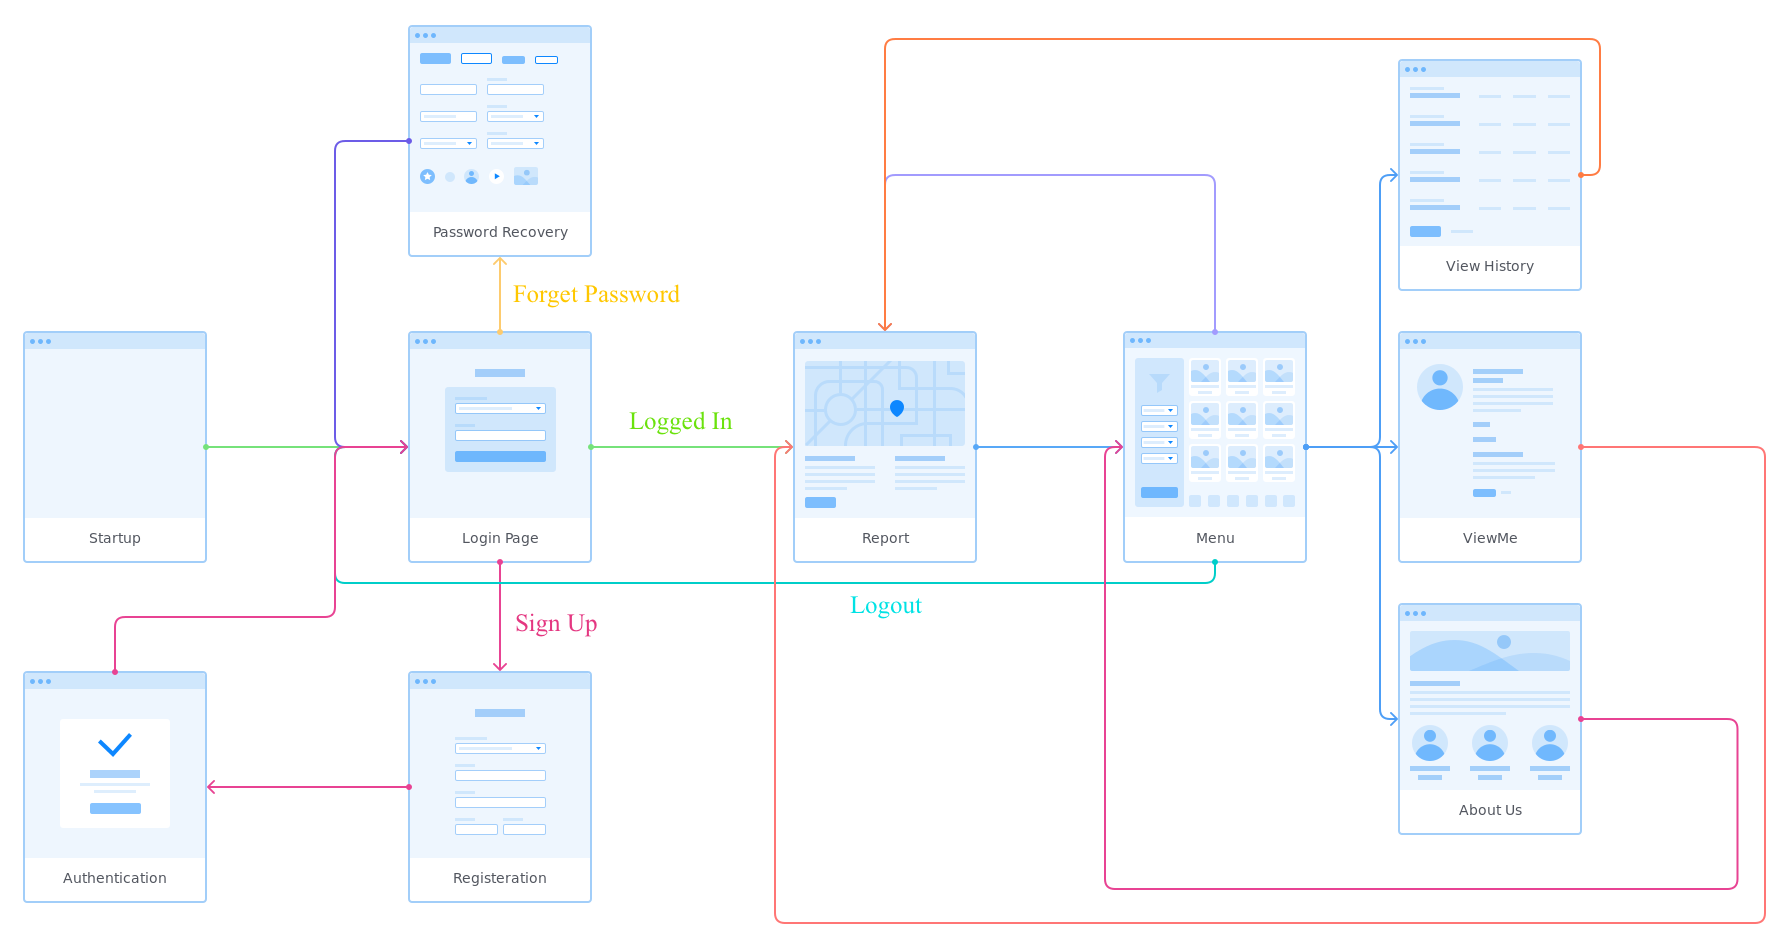
\includegraphics[width=0.75\linewidth]{UXdiagram.png}
\end{figure}
\end{sidewaysfigure}

